% 04-supervised-learning-classification.tex

% Supervised Learning – Classification
% 4.1. Introduction: Provides an overview of the supervised learning task and its objectives.
% 4.2. Data Splitting: Describes the process of splitting the dataset into training and test sets.
% 4.3. Baseline Model Implementation: Implements and evaluates baseline models.
% 4.4. Hyperparameter Tuning: Tunes hyperparameters and evaluates performance.
% 4.5. Result Analysis: Analyzes the results for each intent.
% 4.6. Feature Experimentation: Explores different feature combinations and their impact on performance.

% Section Title
\section{SUPERVISED LEARNING - CLASSIFICATION}

    % Main Content

    \subsection{Introduction}
    
        The supervised learning experiment in this project aimed to classify attack sessions into various intent categories derived from the \cooltext{Set\_Fingerprint} column of the dataset. This section explores the use of Random Forest and Support Vector Machines (SVM) as the primary models. The analysis focuses on how these models handle multi-label classification and evaluates their performance using metrics such as weighted F1-scores and confusion matrices.

        This section outlines the model training and evaluation processes, and a detailed discussion of the results obtained. Each model's strengths and weaknesses are analyzed, providing insights into their application to multi-label classification problems.

    \subsection{Data Preprocessing}
    
        To effectively apply supervised learning models, it is crucial to represent the textual data in a numerical format. Raw text cannot be directly processed by most machine learning algorithms, so as we said in the previous section, we transformed the dataset into a structured numerical form.
    
        Unlike BoW, which merely counts word occurrences without differentiating their relevance, TF-IDF downweights frequently occurring words that may not carry significant information (e.g., common command-line syntax) and upweights rare but potentially more meaningful terms. This property helps improve the model's ability to differentiate between different types of attacks and intents.
    
        To prepare the data for supervised learning:

        \begin{enumerate}
    
            \item \textbf{Encoding Intents:}After loading the TF-IDF dataset, the \cooltext{Set\_Fingerprint} column was encoded into multi-label binary format using the MultiLabelBinarizer. Each intent was represented as a binary vector, allowing for simultaneous prediction of multiple labels.
            
            \item \textbf{Splitting the Data:} The dataset was divided into training (70\%), validation (20\%), and testing (10\%) subsets. Stratified splitting was employed to ensure that all intents were well-represented in each subset.
        
        \end{enumerate}

        These steps ensured the dataset was clean, balanced, and ready for supervised learning.

    \subsection{Model Training}
    
        Three models were trained and evaluated using their default configurations to establish baseline performance:

        \subsubsection*{1. Random Forest \\}
        
            % \vspace{0.5em}
        
            The Random Forest model was trained with default parameters, including 100 estimators and unlimited maximum depth. This initial training provided insights into potential overfitting or underfitting issues and served as a benchmark for subsequent tuning.

        \subsubsection*{2. Support Vector Machines (SVM) \\}
        
            % \vspace{0.5em}
        
            SVM was initially trained with default settings using a linear kernel and a regularization parameter \( C = 1 \). The performance was evaluated to assess the model's ability to handle multi-label classification tasks with linearly separable data.

        \subsubsection*{3. Logistic Regression \\}
        
            % \vspace{0.5em}
        
            In order to have another view of the analysis, we performed the training with the logistic regression model. While the model performed well, the results were not as significant as those of RF and SVM, so they will not be discussed in detail in this section (see Appendix).

    \subsection{Evaluation Metrics}
    
        The models were evaluated using the following metrics:
        
        \begin{itemize}
        
            \item \textbf{Accuracy, Precision, Recall}: basic evaluation metrics.
            
            \item \textbf{Confusion Matrices:} Provided insight into true positives, false positives, false negatives, and true negatives for each intent.
            
            \item \textbf{Weighted F1-Scores:} Measured the harmonic mean of precision and recall, with weights proportional to class support.
        
        \end{itemize}

        This evaluation allowed for the identification of baseline performance, highlighting potential areas for improvement through hyperparameter tuning.

    \subsection{Hyperparameter Tuning}
    
        To optimize each model, hyperparameter tuning was performed using a grid search approach. This process aimed to improve performance and address issues of overfitting or underfitting observed in the baseline models:

        \subsubsection*{1. Random Forest \\}
        
            The grid search explored combinations of the number of estimators (50, 100, and 150) and maximum depth (unlimited, 50, and 100). The best-performing configuration was selected based on weighted F1-scores.

        \subsubsection*{2. Support Vector Machines (SVM) \\}
        
            For SVM, the grid search varied the regularization parameter \( C \) (0.01, 0.1, 1, and 10) and the kernel type (linear and RBF). Additional tuning for the RBF kernel included the gamma parameter (scale and auto).

    \subsection{Results and Observations}

        \subsubsection{Random Forest}
            
            \begin{itemize}
        
                \item \textit{Performance Overview with base model}
                
                    \vspace{0.3em}

                    The Random Forest base model showed robust performance, achieving high weighted F1-scores across all intents. However, minor overfitting was observed in intents with smaller sample sizes. Figure~\ref{fig:rf_cm_base} illustrates the confusion matrix for the base model, showing excellent precision and recall for major intents like \textit{Persistence} and \textit{Defense Evasion}.

                \vspace{0.5em}

                \item \textit{Hyperparameter Analysis}
                
                    \vspace{0.3em}

                    Hyperparameter tuning improved the Random Forest model's performance, particularly for minority intents. The optimized model reduced overfitting by limiting tree depth and increasing the number of estimators. Figure~\ref{fig:rf_f1_tuning} highlights the improvement in weighted F1-scores across different configurations.

                \vspace{0.5em}

                \item \textit{Comparative Analysis of Baseline and Optimized Models}
                
                    \vspace{0.3em}

                    Comparing the base and optimized models revealed significant improvements in precision and recall for minority intents. The optimized model maintained high performance for major intents while addressing issues of overfitting. Figure~\ref{fig:rf_cm_opt} presents the confusion matrix for the optimized Random Forest model.
                
            \end{itemize}

        \subsubsection{Support Vector Machines (SVM)}
        
            \begin{itemize}
        
                \item \textit{Performance Overview with base model}
                
                    \vspace{0.3em}

                    The SVM base model performed well for linearly separable data, achieving high precision and recall for intents with large sample sizes. However, it struggled with minority intents due to its sensitivity to class imbalances. Figure~\ref{fig:svm_cm_base} illustrates the confusion matrix for the base model.

                \vspace{0.5em}

                \item \textit{Hyperparameter Analysis}
                
                    \vspace{0.3em}

                    Grid search tuning improved SVM's performance, especially for the RBF kernel. Increasing the regularization parameter \( C \) and fine-tuning the gamma parameter enhanced the model's ability to classify minority intents. Figure~\ref{fig:svm_f1_tuning} shows the weighted F1-scores for different hyperparameter combinations.

                \vspace{0.5em}

                \item \textit{Comparative Analysis of Baseline and Optimized Models}
                
                    \vspace{0.3em}

                    The optimized SVM model outperformed the base model, particularly for minority intents. Figure~\ref{fig:svm_cm_opt} displays the confusion matrix for the optimized model, highlighting the improvements in precision and recall for challenging classifications.

            \end{itemize}

    \subsection{Conclusion} % FIXME: maybe "Conclusion" is not the right word
    
        Random Forest and SVM both demonstrated strong performance in this experiment. Random Forest's ensemble nature provided robustness and generalization, making it the best-performing model overall. SVM, particularly with the linear kernel, offered comparable results but required more tuning to handle imbalanced classes effectively. These findings highlight the importance of selecting models and hyperparameters tailored to the dataset's characteristics and the problem's requirements.     
        
        
    % Plot pages
        
        \clearpage

        % Random Forest
        
        \begin{figure}[H]
        
            \centering
            
            % Top row
            \begin{minipage}{\textwidth}
                \centering
                \begin{minipage}[c]{\textwidth}
                    \centering
                    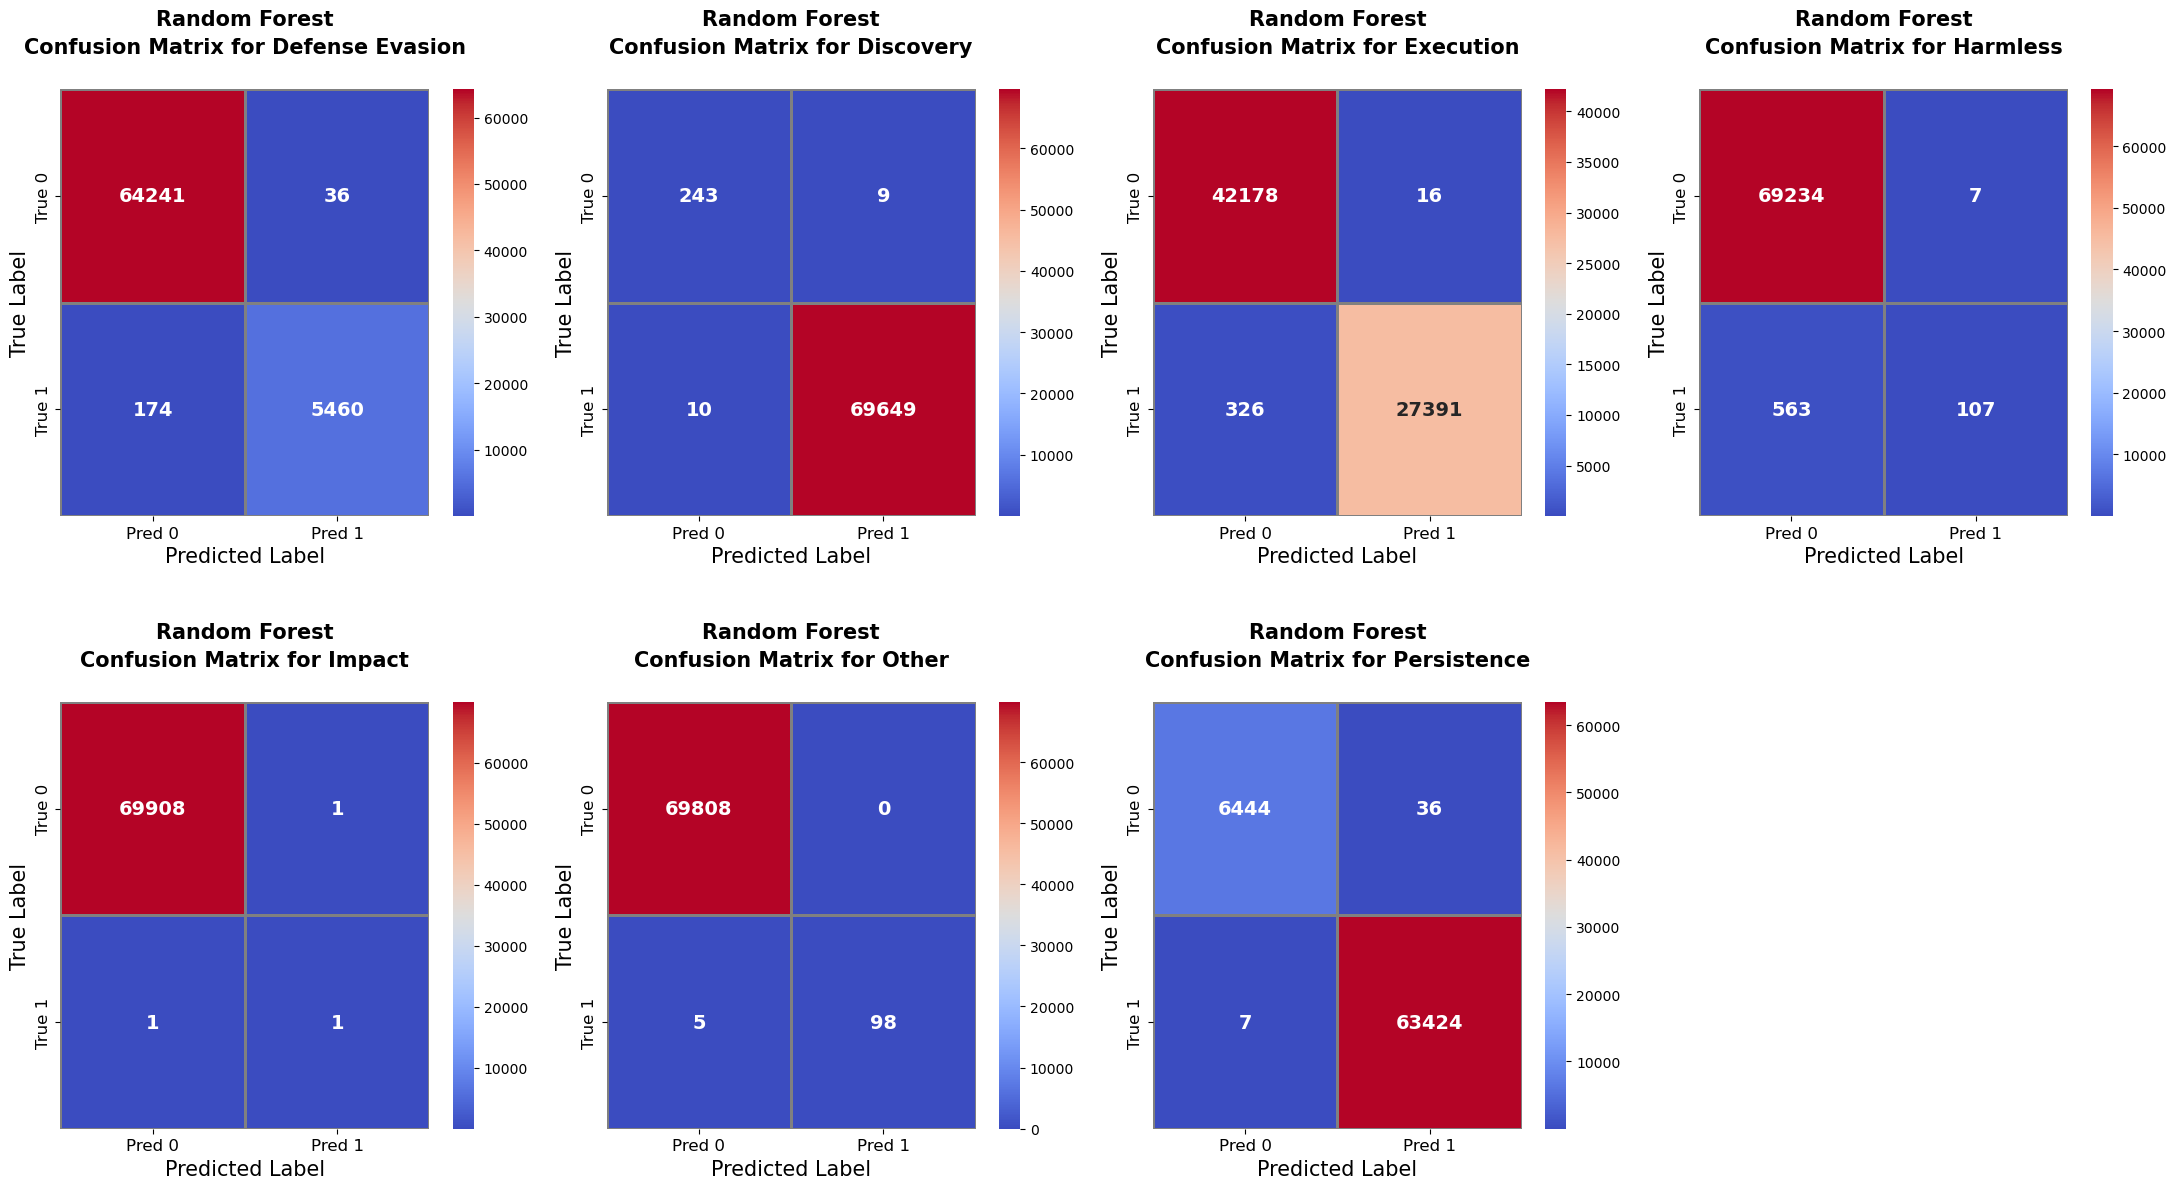
\includegraphics[width=0.75\textwidth]{../figures/plots/section2/Random_Forest_confusion_matrices.png}
                    \caption{Random Forest Confusion Matrices}
                    \label{fig:}
                \end{minipage}%
            \end{minipage}

            \vspace{0.5cm}  % Add some vertical spacing between rows
            
            % Middle row  
            \begin{minipage}{\textwidth}
                % Middle-left (Train)
                \begin{minipage}[c]{0.48\textwidth}
                    \centering
                    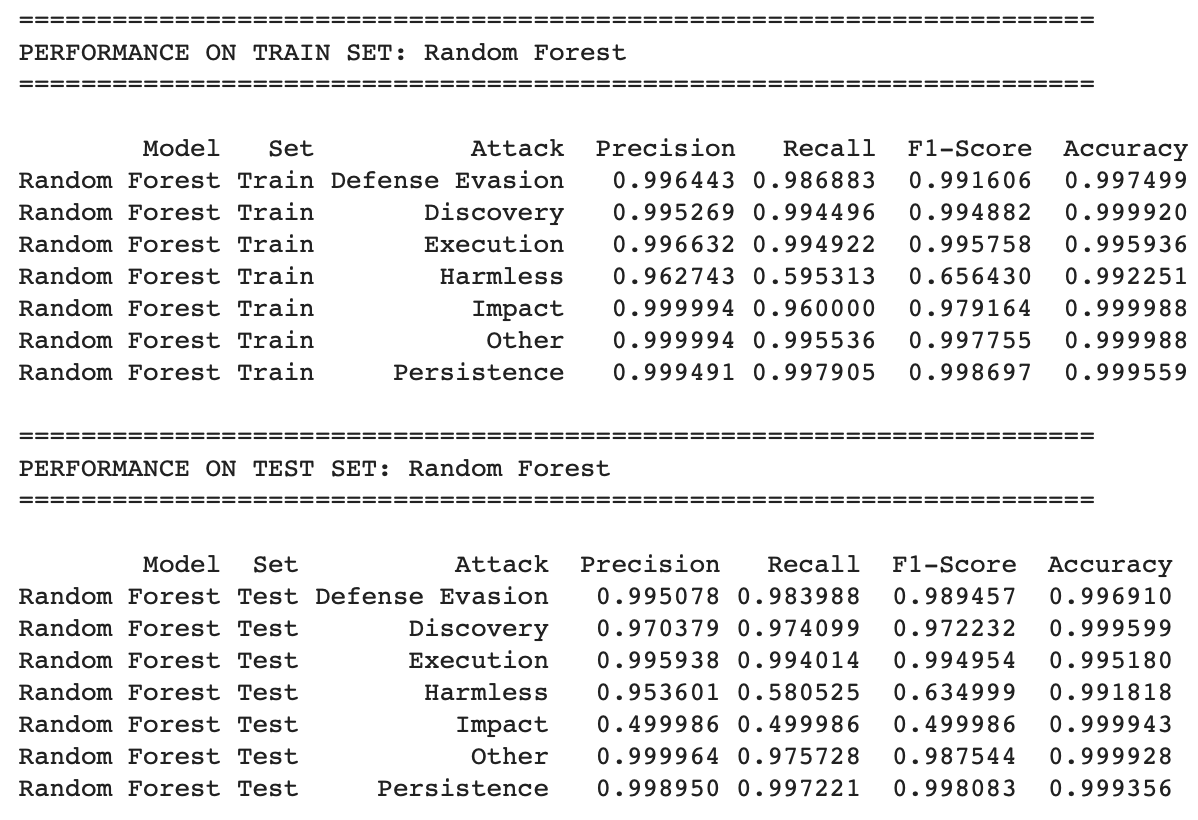
\includegraphics[width=0.9\textwidth]{../figures/plots/section2/Random_Forest_evaluation_metrics_1.png}
                    \caption{Random Forest Evaluation Metrics}
                    \label{fig:}
                \end{minipage}%
                \hfill%
                % Middle-right (Train)
                \begin{minipage}[c]{0.48\textwidth}
                    \centering
                    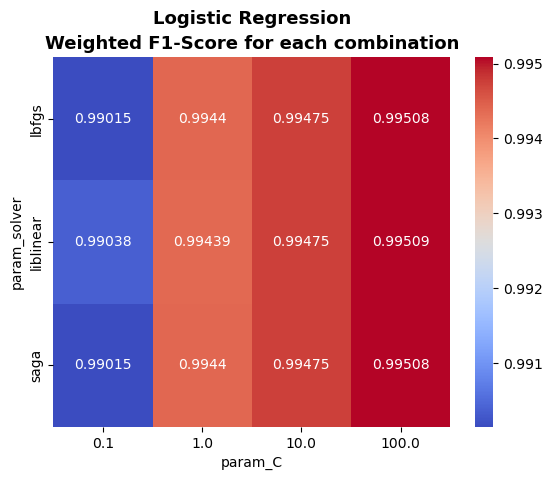
\includegraphics[width=0.7\textwidth]{../figures/plots/section2/weighted_f1_score_for_each_combination_of_parameters_logistic_regression.png}
                    \caption{Random Forest Weighted F1 Scores}
                    \label{fig:}
                \end{minipage}
            \end{minipage}
            
            \vspace{0.5cm}  % Add some vertical spacing between rows

            % Bottom row
            \begin{minipage}{\textwidth}
                % Bottom-left (Test)
                \begin{minipage}[t]{0.48\textwidth}
                    \centering
                    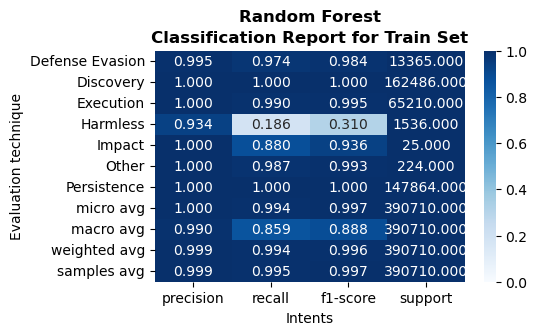
\includegraphics[width=0.9\textwidth]{../figures/plots/section2/Random Forest_classification_report_for_Train_set.png}
                    \caption{Random Forest Classification Report Train Set}
                    \label{fig:}
                \end{minipage}%
                \hfill%
                % Bottom-right (Test)
                \begin{minipage}[t]{0.48\textwidth}
                    \centering
                    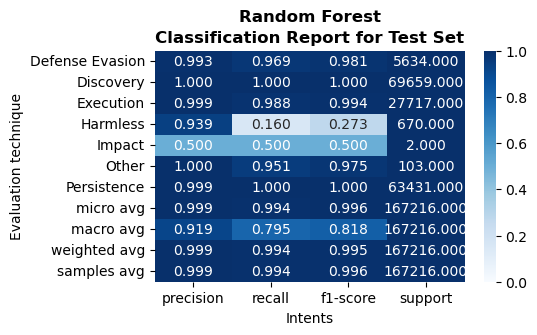
\includegraphics[width=0.9\textwidth]{../figures/plots/section2/Random Forest_classification_report_for_Test_set.png}
                    \caption{Random Forest Classification Report Test Set}
                    \label{fig:}
                \end{minipage}  
            
            \end{minipage}
            
        \end{figure}
            
        \clearpage
    
        % SVM
        
        \begin{figure}[H]
        
            \centering
            
            % Top row
            \begin{minipage}{\textwidth}
                \centering
                \begin{minipage}[c]{\textwidth}
                    \centering
                    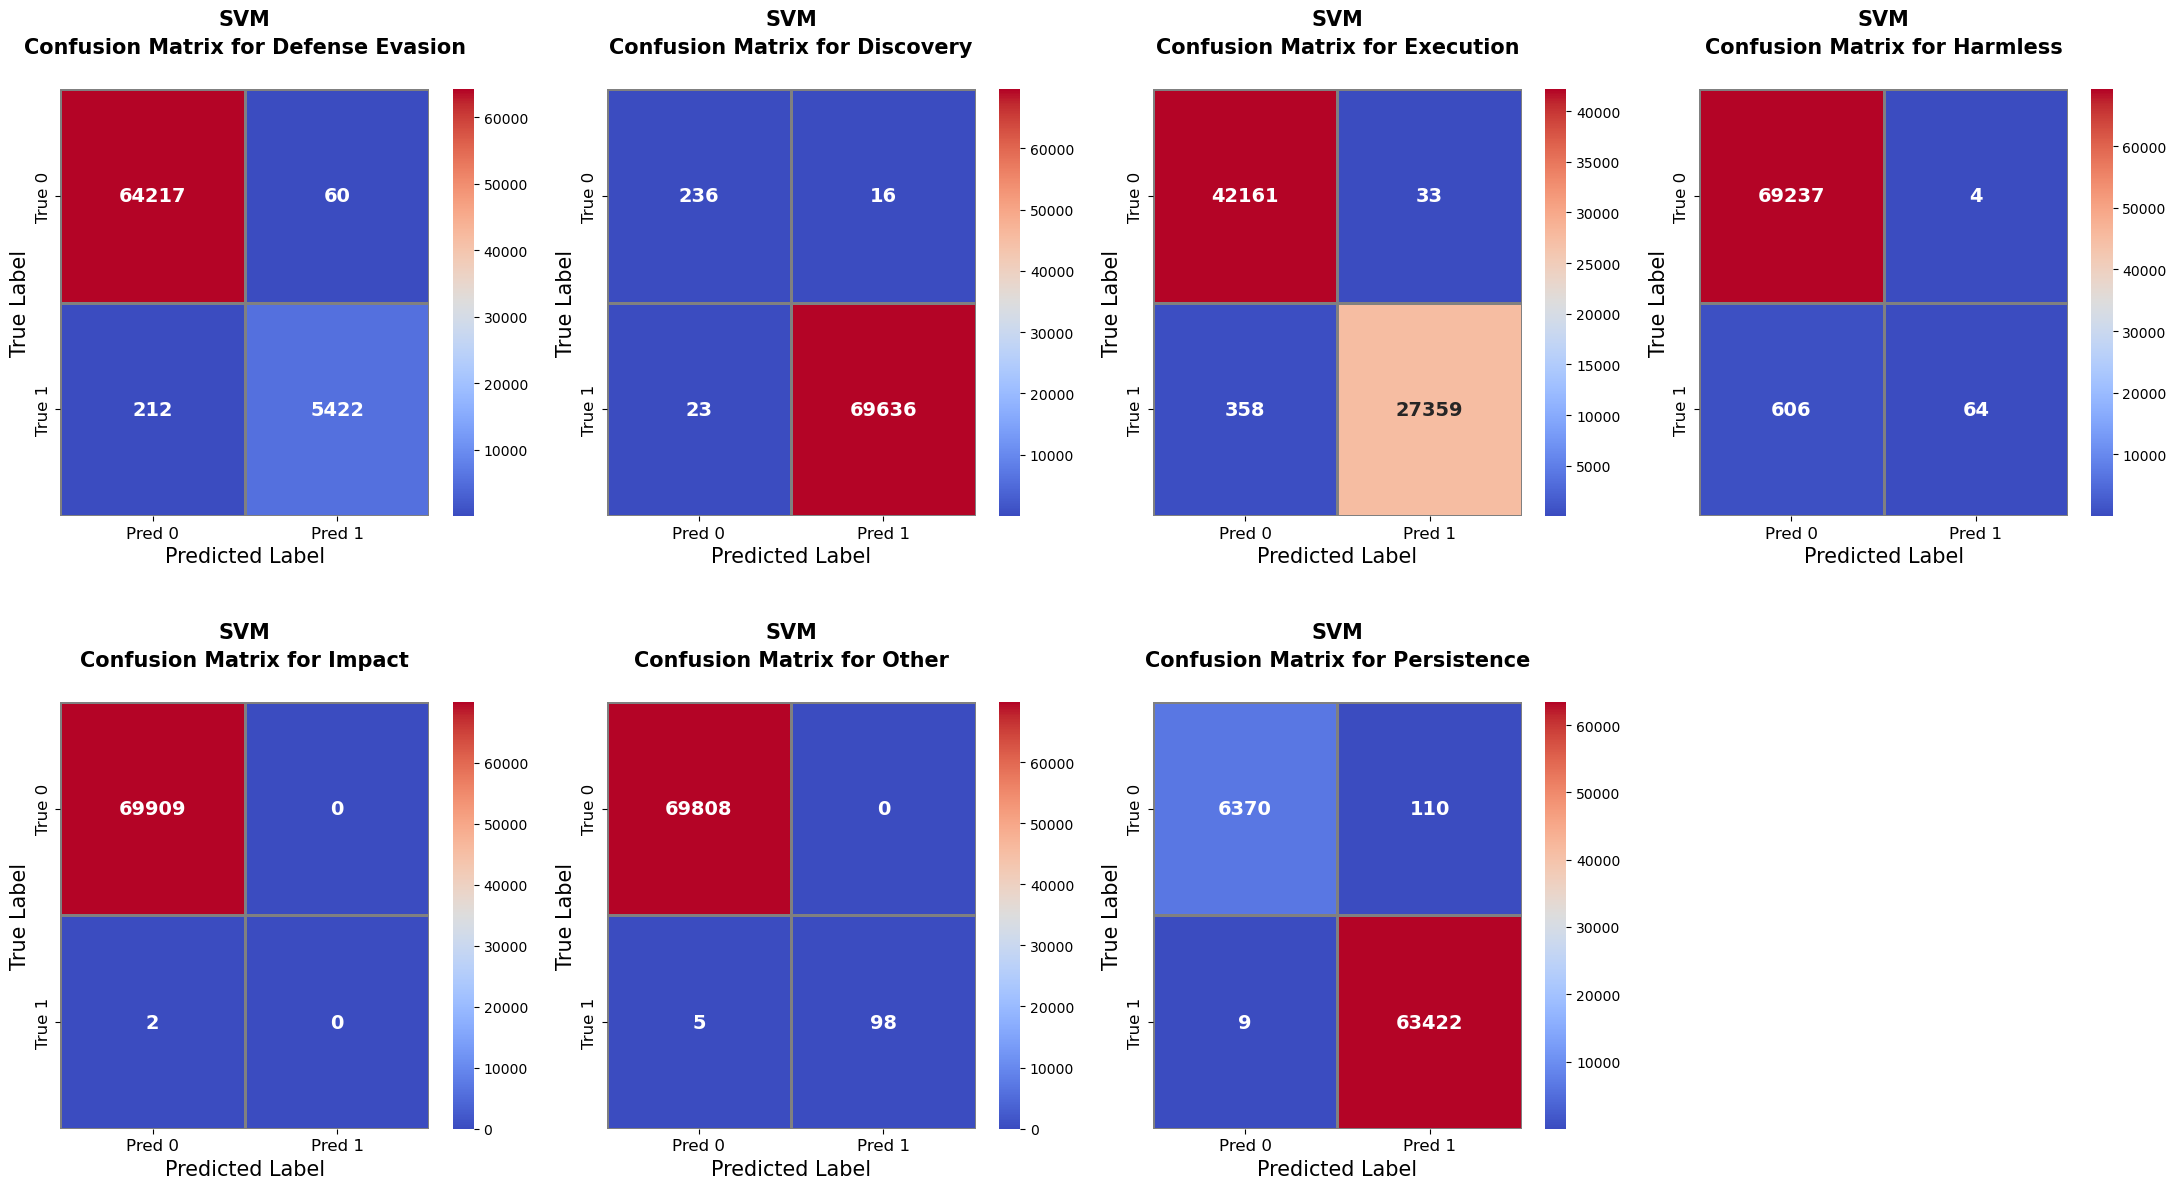
\includegraphics[width=0.75\textwidth]{../figures/plots/section2/SVM_confusion_matrices.png}
                    \caption{SVM Confusion Matrices}
                    \label{fig:}
                \end{minipage}%
            \end{minipage}

            \vspace{0.5cm}  % Add some vertical spacing between rows
            
            % Middle row  
            \begin{minipage}{\textwidth}
                % Middle-left (Train)
                \begin{minipage}[c]{0.48\textwidth}
                    \centering
                    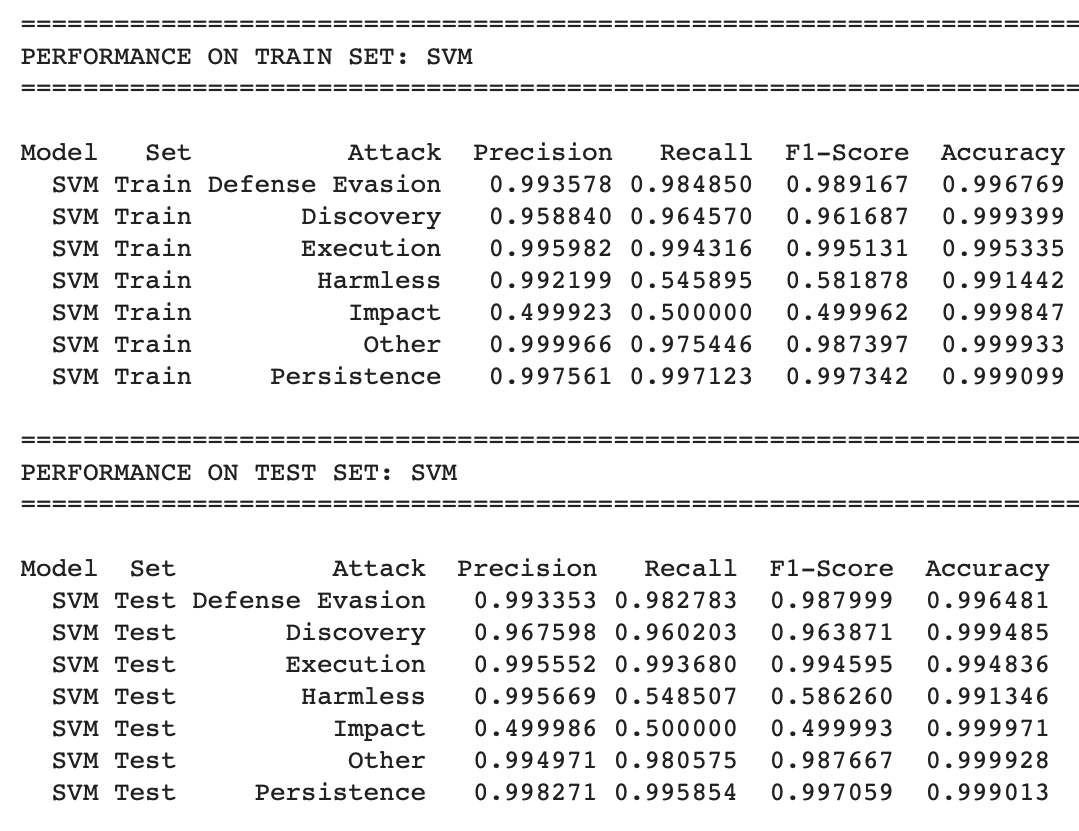
\includegraphics[width=0.8\textwidth]{../figures/plots/section2/SVM_evaluation_metrics_1.png}
                    \caption{SVM Evaluation Metrics}
                    \label{fig:}
                \end{minipage}%
                \hfill%
                % Middle-right (Train)
                \begin{minipage}[c]{0.48\textwidth}
                    \centering
                    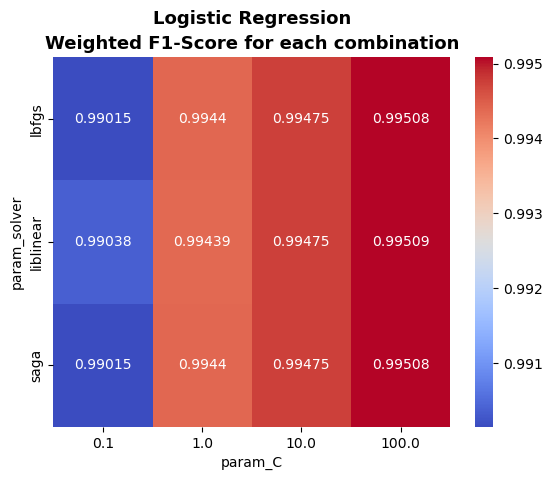
\includegraphics[width=0.7\textwidth]{../figures/plots/section2/weighted_f1_score_for_each_combination_of_parameters_logistic_regression.png}
                    \caption{SVM Weighted F1 Scores}
                    \label{fig:}
                \end{minipage}
            \end{minipage}
            
            \vspace{0.5cm}  % Add some vertical spacing between rows

            % Bottom row
            \begin{minipage}{\textwidth}
                % Bottom-left (Test)
                \begin{minipage}[t]{0.48\textwidth}
                    \centering
                    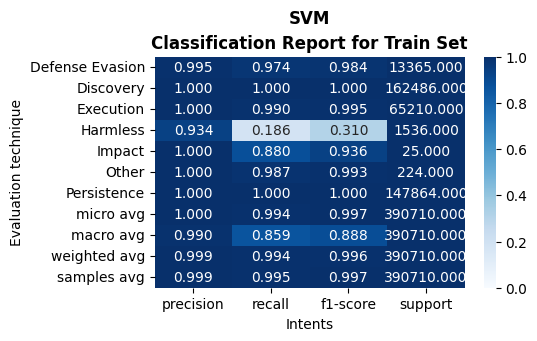
\includegraphics[width=0.9\textwidth]{../figures/plots/section2/SVM_classification_report_for_Train_set.png}
                    \caption{SVM Classification Report Train Set}
                    \label{fig:}
                \end{minipage}%
                \hfill%
                % Bottom-right (Test)
                \begin{minipage}[t]{0.48\textwidth}
                    \centering
                    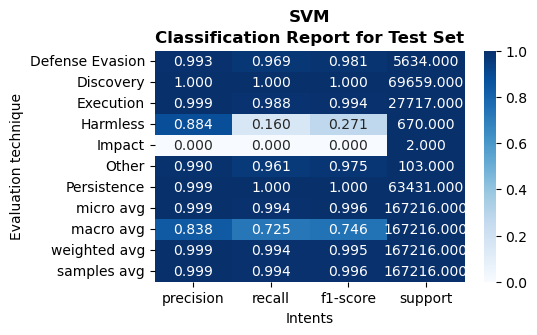
\includegraphics[width=0.9\textwidth]{../figures/plots/section2/SVM_classification_report_for_Test_set.png}
                    \caption{SVM Classification Report Test Set}
                    \label{fig:}
                \end{minipage}  
            
            \end{minipage}
            
        \end{figure}
